\chapter{Additional Information on the Simulation with Rebalancing}\label{appendix:additional_info_reba}


	

\begin{figure}[th]
	\centering
	\begin{subfigure}[b]{0.35\textwidth}
		\centering
		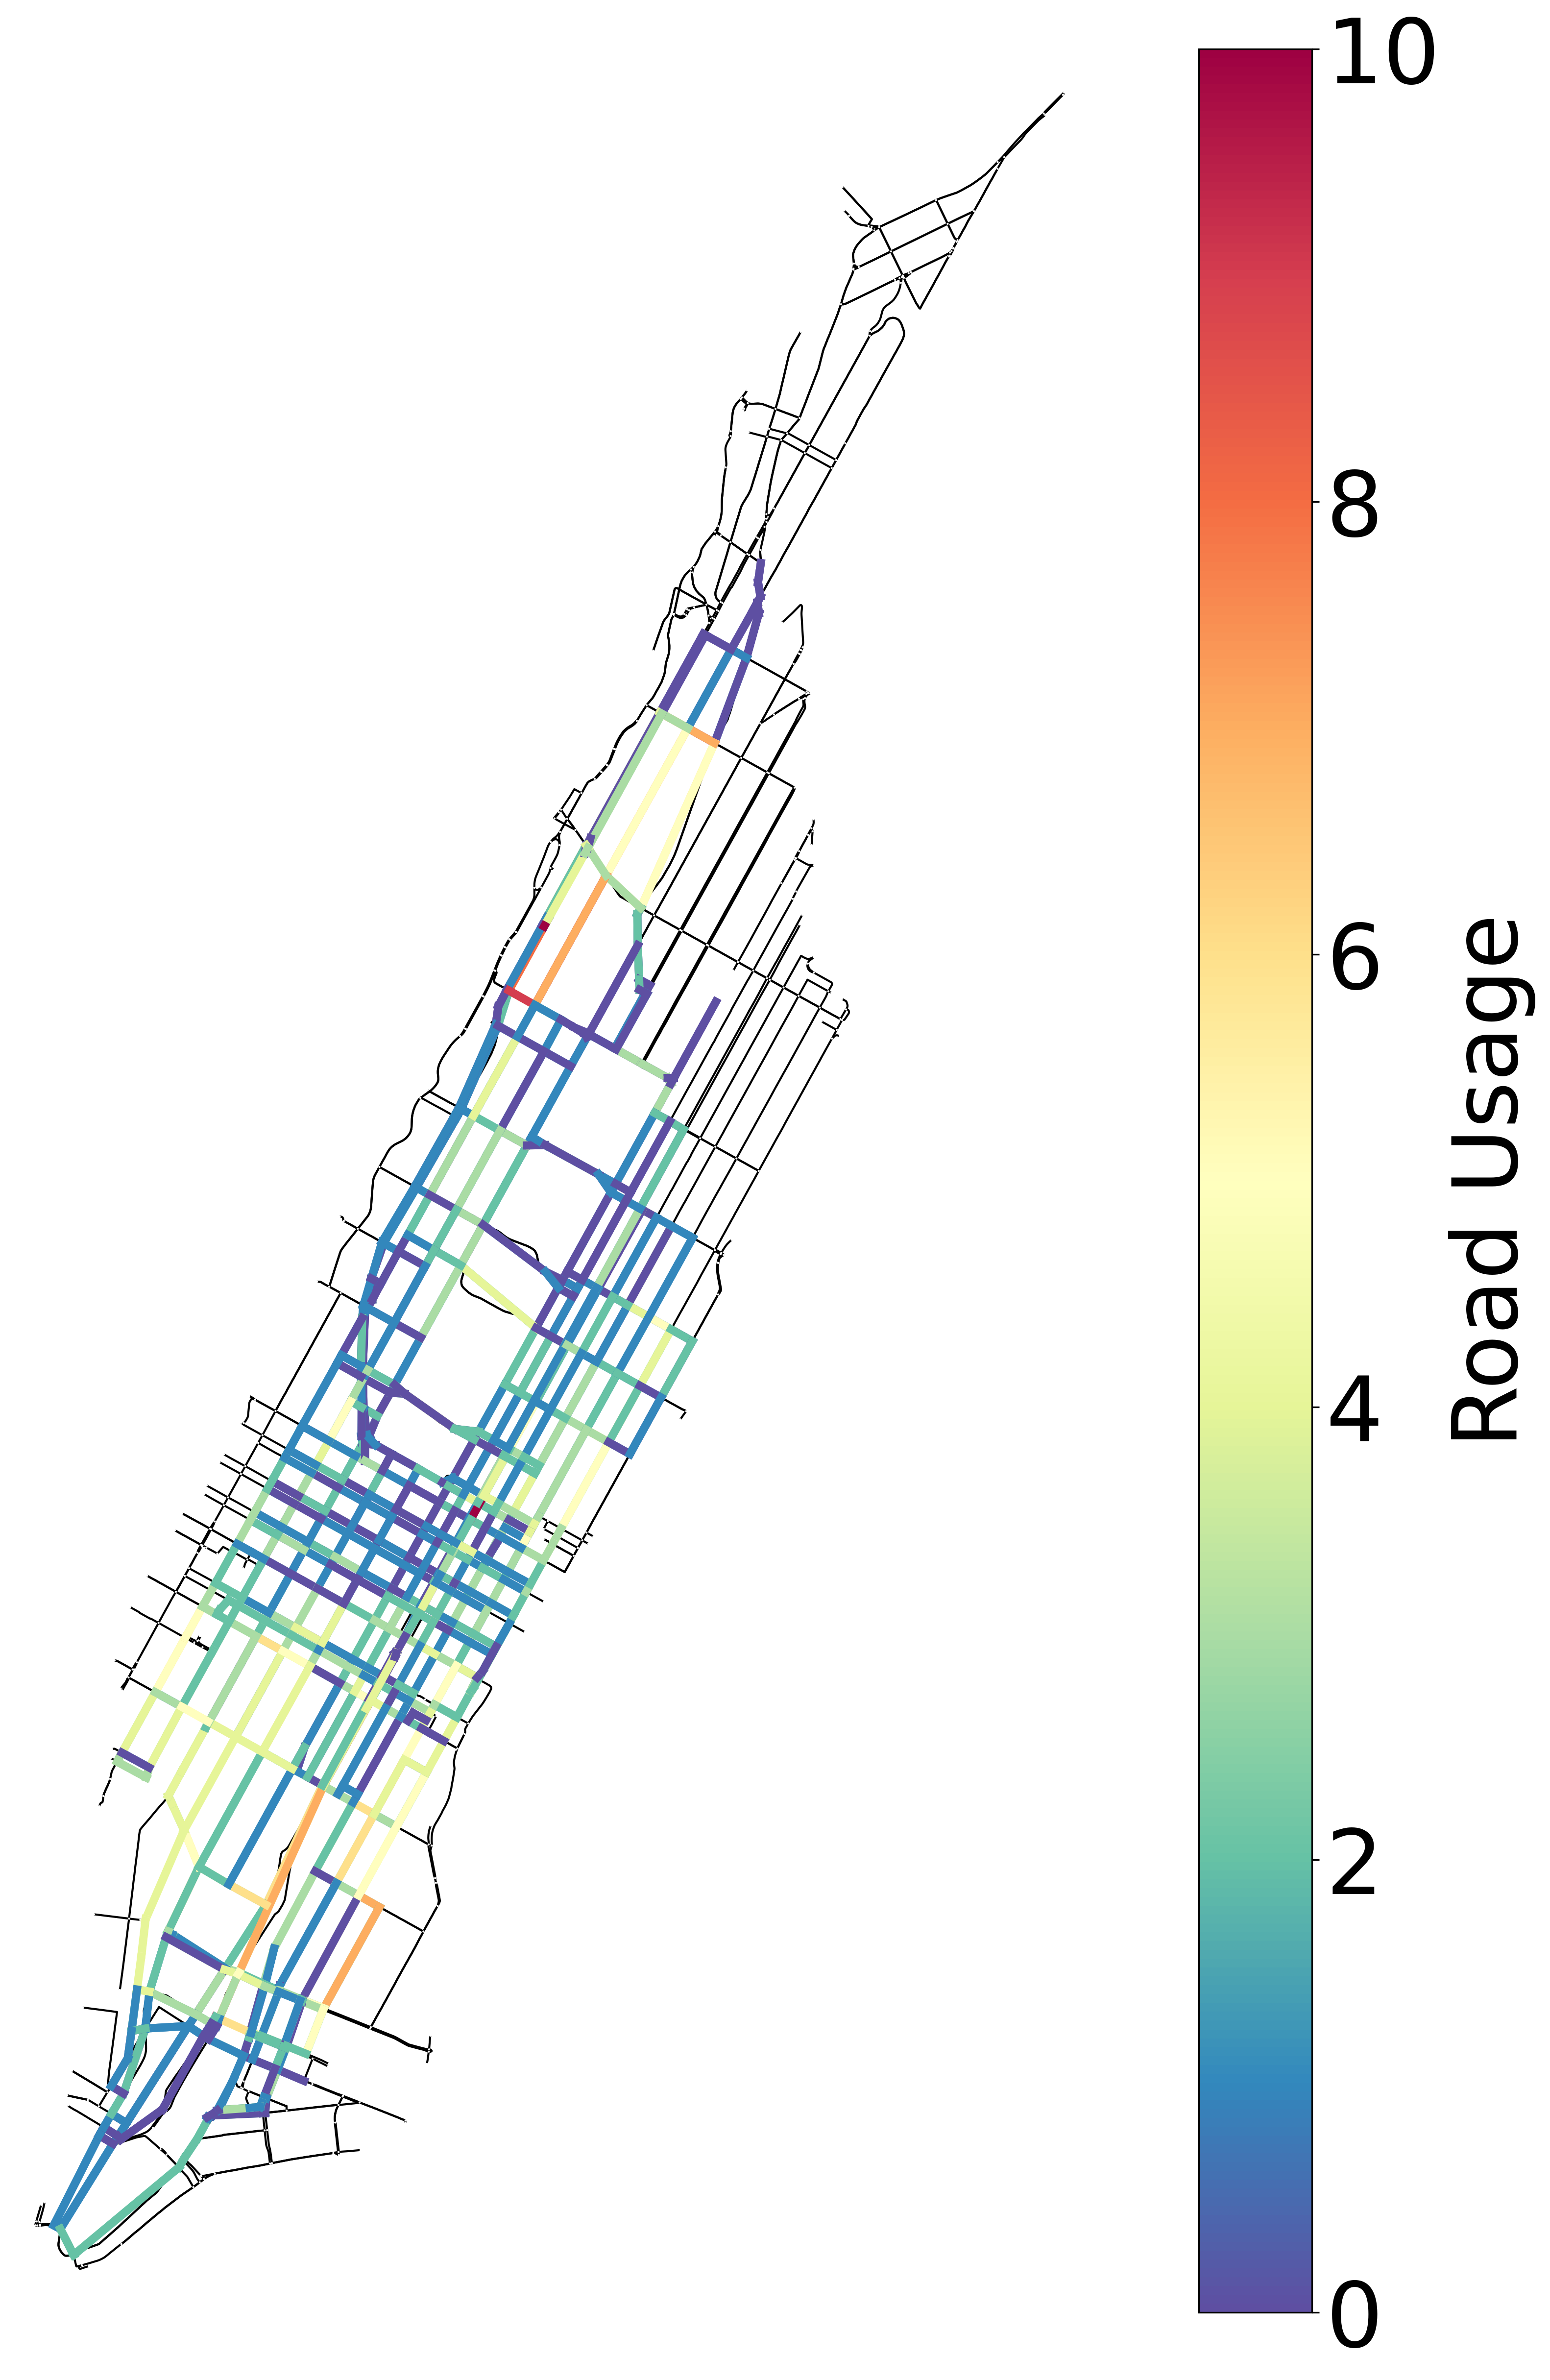
\includegraphics[width=\textwidth]{assets/img/07_graph_based/nyc_road_usage_rebalancing_simu_1.png}
		\caption{}
		\label{fig:nyc_road_usage_rebalancing_simu_1}
	\end{subfigure}
	\begin{subfigure}{0.5\textwidth}
		\begin{tikzpicture}
			\begin{axis}[
				xlabel={Iteration},
				ylabel={Charge (\%)},
				xtick={0,1,2,3,4,5,6,7,8,9,10},
				width=7cm,
				ytick = {20,40,60,80,100},
				%legend pos=north west,
				legend style={at={(1.05,1)},anchor=north west},
				ymajorgrids=true,
				grid style=dashed,
				thick,
				]
				
				\addplot[color = viridisbluecolor]
				coordinates {
					(0,100.0)
					(1,62.59510042230054)
					(2,100.0)
					(3,100.0)
					(4,100.0)
					(5,46.903863217746256)
					(6,100.0)
					(7,100.0)
					(8,97.17818508556614)
					(9,73.7749920645868)
				};
				\addplot[color = viridisyellowcolor]
				coordinates {
					(0,100.0)
					(1,97.17818508556614)
					(2,100.0)
					(3,100.0)
					(4,100.0)
					(5,100.0)
					(6,100.0)
					(7,60.87675184062758)
					(8,100.0)
					(9,100.0)
				};
				\addplot[color= viridisgreencolor]
				coordinates {
					(0,89.08968460550663)
					(1,100.0)
					(2,100.0)
					(3,100.0)
					(4,79.47835078320651)
					(5,100.0)
					(6,100.0)
					(7,100.0)
					(8,48.36639730450669)
					(9,100.0)
				};
				
				\addplot[color= viridisorangecolor]
				coordinates {
					(1,100.0)
					(2,100.0)
					(3,100.0)
					(4,44.28939805640962)
					(5,100.0)
					(6,42.42226432775283)
					(7,100.0)
					(8,82.47179903200924)
					(9,95.22271835395512)
				};
				
				\addplot[ color = viridispurplecolor]
				coordinates {
					(0,100.0)
					(1,100.0)
					(2,18.21615357519943)
					(3,78.21615357519943)
					(4,100.0)
					(5,100.0)
					(6,91.9546)
					(7,97.17818508556614)
					(8,100.0)
					(9,91.386258)
				};
				
				\legend{3,4,5,6,17}
			\end{axis}
			
		\end{tikzpicture}
		\caption{}
		\label{fig:ex_soc_vehicles_rebalancing_simu_1}
	\end{subfigure}
	
	\caption{Road Usage and State of Charge of an exemplary Set of Vehicles for the Simulation 1 with Rebalancing}
	\label{fig:ex_soc_rebalancing_simu_1}
\end{figure}



\begin{figure}[th]
	\centering
	\begin{subfigure}[b]{0.35\textwidth}
		\centering
		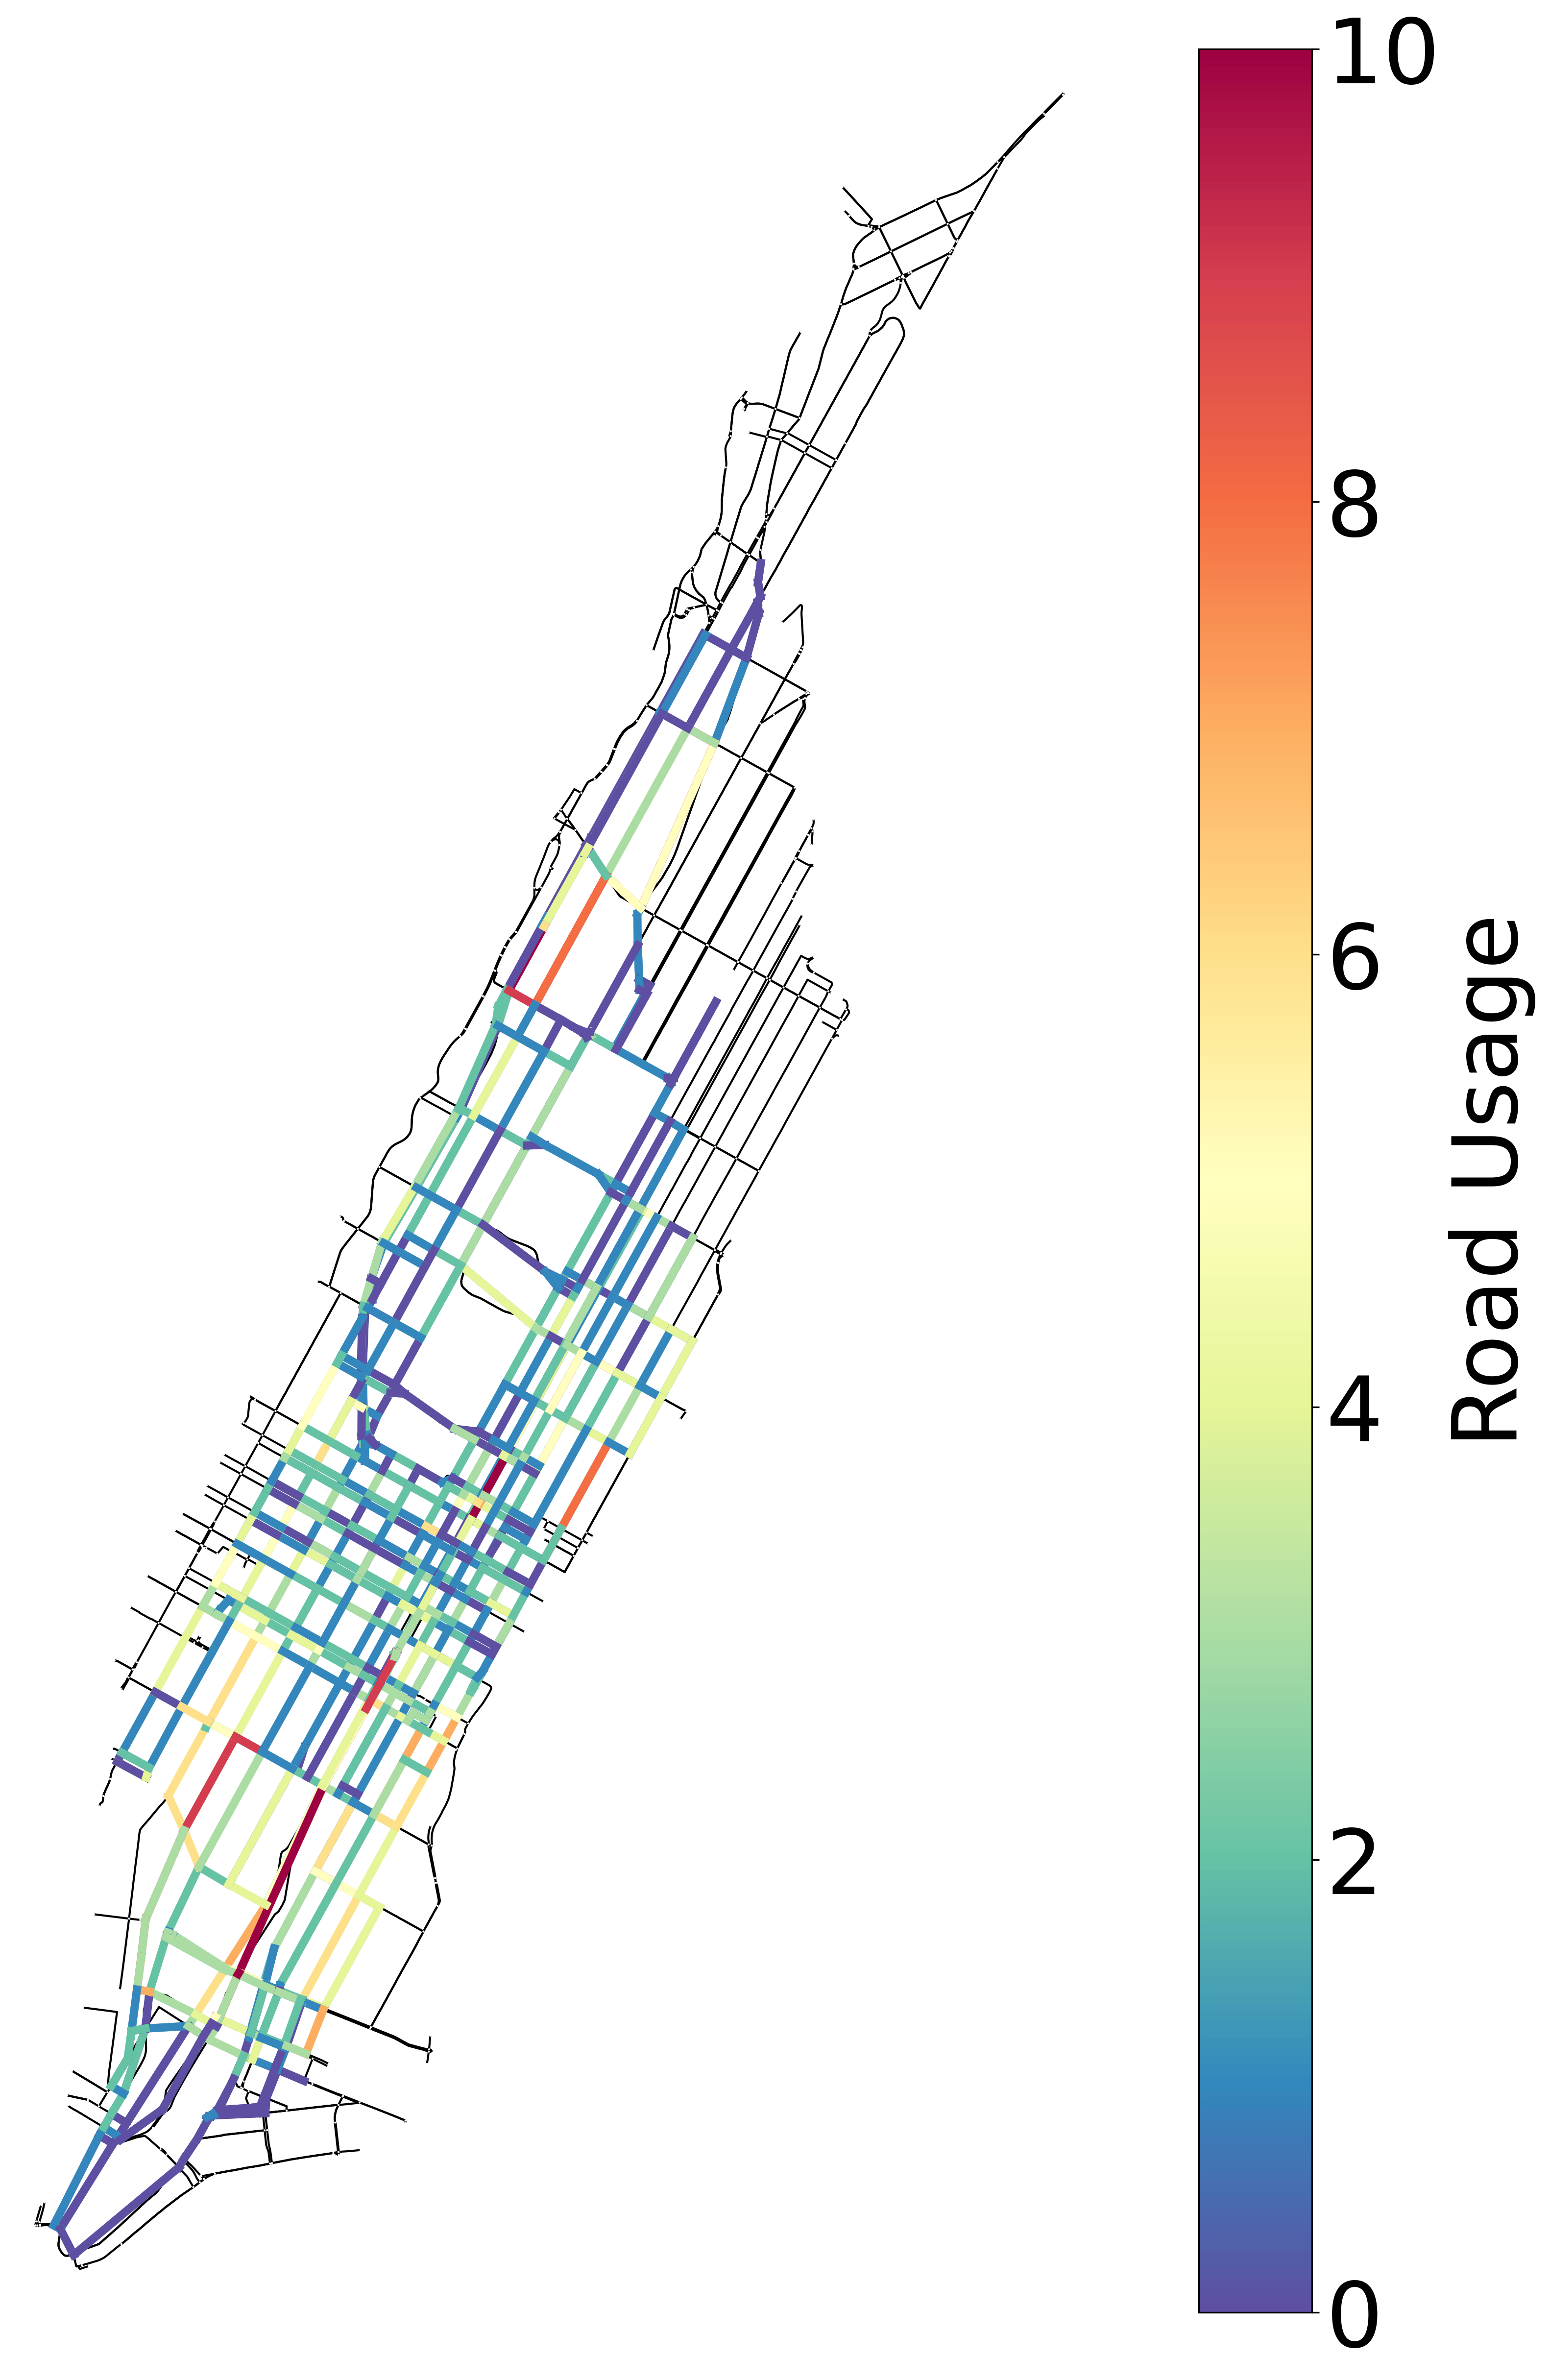
\includegraphics[width=\textwidth]{assets/img/07_graph_based/nyc_road_usage_simu_4.png}
		\caption{}
		\label{fig:nyc_road_usage_rebalancing_simu_4}
	\end{subfigure}
	\begin{subfigure}{0.5\textwidth}
		\begin{tikzpicture}
			\begin{axis}[
				xlabel={Iteration},
				ylabel={Charge (\%)},
				xtick={0,1,2,3,4,5,6,7,8,9,10},
				ytick = {20,40,60,80,100},
				width=7cm,
				%legend pos=north west,
				legend style={at={(1.05,1)},anchor=north west},
				ymajorgrids=true,
				grid style=dashed,
				thick,
				]
				
				\addplot[color = viridisbluecolor]
				coordinates {
					(0,3.780043567190811)
					(1,33.78004356719081)
					(2,63.78004356719081)
					(3,93.7800435671908)
					(4,57.73975766312199)
					(5,58.83407213532249)
					(6,41.37168379516582)
					(7,71.37168379516582)
					(8,90.58239512581032)
					(9,100.0)
				};
				\addplot[color = viridisyellowcolor]
				coordinates {
					(0,20.01370958236381)
					(1,50.01370958236381)
					(2,80.01370958236382)
					(3,38.29016303811425)
					(4,68.29016303811426)
					(5,95.4683481236804)
					(6,100.0)
					(7,100.0)
					(8,100.0)
					(9,100.0)
				};
				\addplot[color= viridisgreencolor]
				coordinates {
					(0,70.25496782523537)
					(1,100.0)
					(2,100.0)
					(3,100.0)
					(4,63.14125109601946)
					(5,93.14125109601946)
					(6,65.38104039418934)
					(7,95.38104039418934)
					(8,100.0)
					(9,61.13385500018325)
				};
				
				\addplot[color= viridisorangecolor]
				coordinates {
					(0,100.0)
					(1,100.0)
					(2,100.0)
					(3,100.0)
					(4,100.0)
					(5,100.0)
					(6,100.0)
					(7,100.0)
					(8,100.0)
					(9,45.51089458924196)
				};
				
				\addplot[ color = viridispurplecolor]
				coordinates {
					(0,100.0)
					(1,100.0)
					(2,65.58711780281972)
					(3,95.58711780281972)
					(4,100.0)
					(5,100.0)
					(6,100.0)
					(7,100.0)
					(8,94.23546)
					(9,100.0)
				};
				
				\legend{0,3,5,10,13}
			\end{axis}
			
		\end{tikzpicture}
		\caption{}
		\label{fig:ex_soc_vehicles_rebalancing_simu_4}
	\end{subfigure}
	
	\caption{Road Usage and State of Charge of an exemplary Set of Vehicles for the Simulation 4 with Rebalancing}
	\label{fig:ex_soc_rebalancing_simu_4}
\end{figure}

